\chapter{Introduction}\label{chapter:introduction}

\section{Background information on blockchain}\label{sec:}
\section{Background information on decentralized applications (dApps)}\label{sec:}
\section{Research question / motivation}\label{sec:}
\section{Thesis organization}\label{sec:organization}



% \indent write here


% \begin{figure}[h]
%     \begin{minipage}{0.5\textwidth}
%         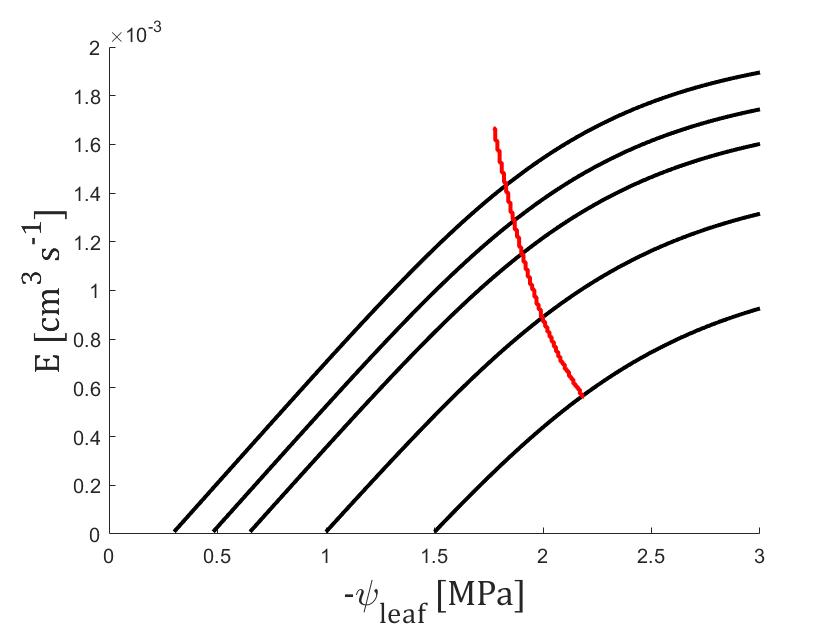
\includegraphics[width=0.9\linewidth, height=6cm]{./img/1_intro/random_figure.jpg}
%     \end{minipage}
%     \hfill
%     \begin{minipage}{0.5\textwidth}
%         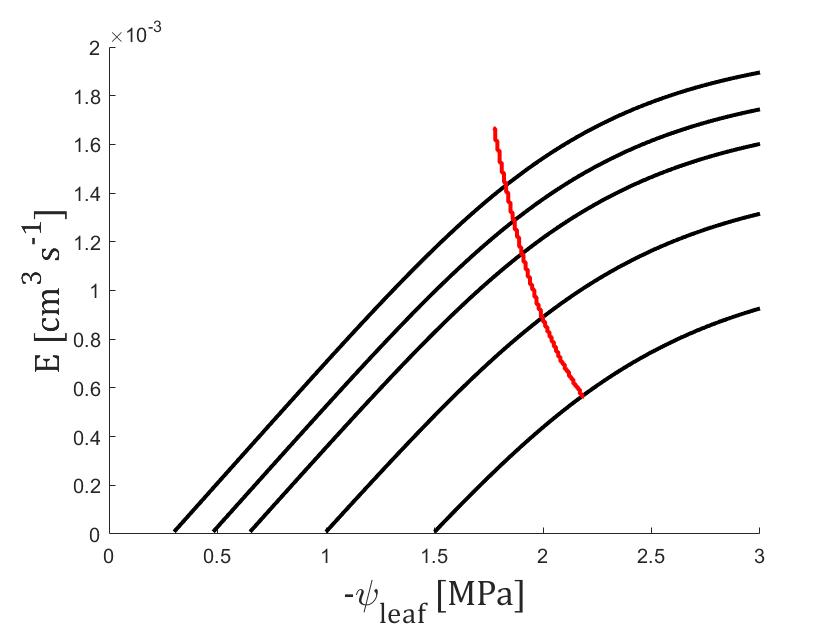
\includegraphics[width=1\linewidth, height=6cm]{./img/1_intro/random_figure.jpg}
%     \end{minipage}
%     \caption{If you want two figures next to each other}
%     \label{Figure:conceptually}
% \end{figure}

% or if you want just one 

% \begin{figure}[h]
%     \centering
%     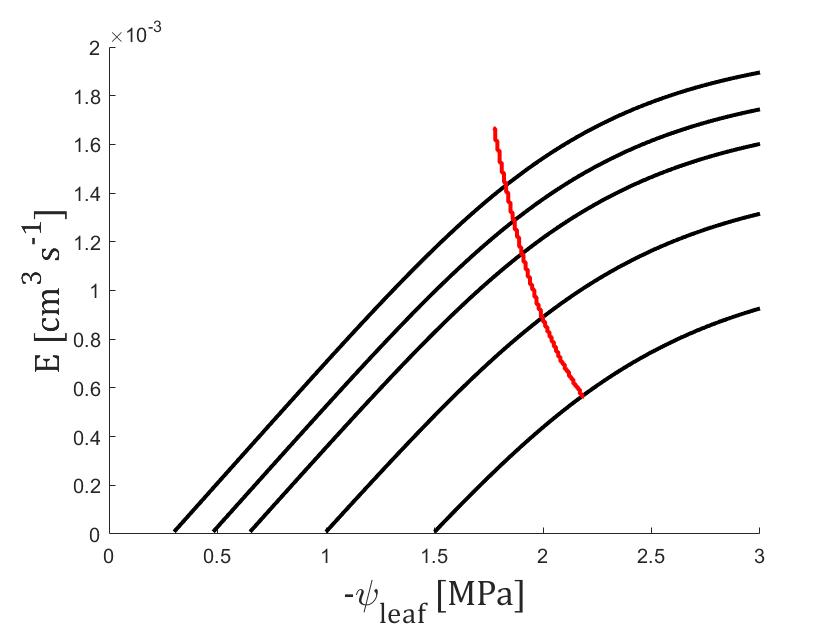
\includegraphics[width=0.5\linewidth, height=5cm]{./img/1_intro/random_figure.jpg}
%     \caption{If you want just one }
%     \label{Figure:just one }
% \end{figure}

% and you can reference it like this \ref{Figure:just one }

% \begin{table}[!h]
% \begin{center}
% \begin{tabular}{llcr} 
% \toprule
% & \textbf{parameter} & \textbf{type 1 } & \textbf{type 2 }\\
%  \midrule
%  \si{k_{0}}  & something & \SI{2e-05}{cm s^{-1}} &\SI{1e-03}{cm s^{-1}}\\
%   \si{h_{0}}  & other thing & \SI{-27.8}{cm} & \SI{-34.5}{cm}\\ 
%   \si{\tau} & exponent & 2 & 3 \\

% \bottomrule
% \end{tabular}
% \caption{This is how you make a table}
% \end{center}
% \end{table}
